\pdfoutput=1
% In particular, the hyperref package requires pdfLaTeX in order to break URLs across lines.

\documentclass[11pt]{article}

% Remove the "review" option to generate the final version.
\usepackage[review]{ACL2023}

% Standard package includes
\usepackage{times}
\usepackage{latexsym}

% For proper rendering and hyphenation of words containing Latin characters
% (including in bib files)
\usepackage[T1]{fontenc}
% For Vietnamese characters
% \usepackage[T5]{fontenc}
% See https://www.latex-project.org/help/documentation/encguide.pdf for other
% character sets

% This assumes your files are encoded as UTF8
\usepackage[utf8]{inputenc}

% This is not strictly necessary, and may be commented out.
% However, it will improve the layout of the manuscript,
% and will typically save some space.
\usepackage{microtype}

% This is also not strictly necessary, and may be commented out.
% However, it will improve the aesthetics of text in
% the typewriter font.
\usepackage{inconsolata}
\usepackage{graphicx}
\usepackage{amsmath}
\usepackage{amssymb}

% If the title and author information does not fit in the area allocated,
% uncomment the following
%
%\setlength\titlebox{<dim>}
%
% and set <dim> to something 5cm or larger.

% Tables
\usepackage{booktabs}
\usepackage{multirow}

% Urls
\usepackage{hyperref}

% % For naming embeddings
% \newcommand{ }[1]{\texttt{#1}}

% % For naming classifiers
% \newcommand{\Cls}[1]{\texttt{#1}}

% % For naming transformations
% \newcommand{  }[1]{\textsl{`#1'}}

\title{Unveiling Semantic Information in Sentence Embeddings}

\author{David Burian^1 \And Vojtěch John^1 \And Leixin Zhang^2 \And Ondřej             Bojar^1\\}
 \\
   % Faculty Of Mathematics and Physics, Charles University^1\\
   % Seminar für Sprachwissenschaft, Universität Tübingen^2\\
   %      }

%     Computational Linguistics\\
%     Seminar für Sprachwissenschaft,
%     Universität Tübingen, Germany \\ 
%     \texttt{leixin.zhang@student.uni-tuebingen.de}
%     }
% \author{David Burian\\
%   Charles University, Prague\\
%   \texttt{david.burian@matfyz.cz}
%   }
% \author{Vojtěch John\\
%  Charles University, Prague\\
%  }


\begin{document}
\maketitle

\begin{abstract}

This study evaluates the extent to which semantic information is preserved within sentence embeddings trained with doc2vec and SBERT. 
Specifically, we examined whether sentence embeddings within one class, (e.g., `formal sentence') exhibit similarities and cluster together in high dimensional space, and whether they are separable from embeddings of other classes such as `nonsense'.  Our experiments suggest that embeddings trained by SBERT achieve positive performance, but doc2vec does not show a comparable outcome. Additionally, we observe variations in performance across different classes. Notably, tense-related classes (e.g., `future' and `past') and classes containing specific keywords (e.g., negative imperative) demonstrate higher separability in clustering tests and greater predictability in classification tests.
\end{abstract}

\section{Introduction}

Word embeddings are commonly used as input in deep neural networks. However, representing an entire sentence numerically, specifically, as a vector of a fixed length poses significant challenges. Similarly, there is a need for further research to assess the capacity of sentence embeddings in capturing the semantic information of a sentence.


The challenges arise from both training and assessment of sentence embeddings. Firstly, generating embeddings is not as easy as extracting word embeddings from a text based on the surrounding context. Sentence embeddings can be sparse and less representational. 
On the other hand, evaluating the quality of sentence embeddings is not an easy task. Assessing whether the embeddings capture the meaning of sentences on a large scale requires a human-annotated corpus with well-defined semantic classes or sentence similarity indexes.

In this study,  we convert Czech sentences in Costra corpus into embeddings by using SBERT and  doc2vec models. Costra corpus \cite{baranvcikova2020costra} is a collection of Czech sentences with semantic labels. Each set comprises a `seed' sentence  and other transformation sentences, such as `paraphrase' and `different meaning'. The goal of this study is to assess whether sentence embeddings trained by  SBERT and  doc2vec preserve semantic information in some way and whether embeddings from the same transformation class cluster together and separate from other classes in space. 


The paper is structured as follows: Section \ref{sec:related work} provides an overview of the SBERT and doc2vec, along with a detailed introduction to the Costra corpus. Section \ref{sec: embeddings} presents initial experiments of extracting transformation vectors and visualizing them in 2-D graphs. In Section \ref{sec:cosine}, the extracted transformation embeddings are used to predict original SBERT sentence embeddings, and they are compared using cosine similarity. Section \ref{sec:cluster} implements unsupervised methods to pairwise assess the separability of embeddings from other transformation classes. In Section \ref{sec:classification}, supervised methods are employed to train and predict transformation classes, to investigate whether the semantic information (transformation labels) is preserved in sentence embeddings and can be distinguished through classification methods.


\section{Related Work} \label{sec:related work}

This section introduces the two models, SBERT and doc2vec, that were used in our study to generate sentence embeddings. Subsequently, we provide an overview of the Costra corpus \cite{baranvcikova2020costra}, which serves as the dataset for evaluating the performance of the sentence embeddings.

% SBERT
Sentence BERT or SBERT \cite{reimers2019sentence} aggregates pre-trained word embeddings of BERT \cite{devlin-etal-2019-bert} by taking their arithmetic mean and fine-tuning with siamese and triplet network structures \cite{reimers2019sentence}. The model has shown success in many previous studies.\cite{opitz-frank-2022-sbert,9140343}.

% Doc2vec
Doc2vec, also referred to as paragraph vector \cite{le2014distributed} is designed to convert long texts into embedding representations of a fixed length. The randomly initialized paragraph embeddings are updated by concatenating with three subsequent word embeddings and predicting the following word in the text. In our study, we used an additional dataset of 1 million Czech sentences to train the model and use the trained doc2vec to predict sentence embeddings in the Costra corpus.


% Costra corpus

% Deep dive into the properties of the datsaet
%   - transformation terminology = transformation
%   - contextualized and distance vector to relation vector
%   - types and explanations of transformations
%   - dataset statistics (count of seeds, sentences in total, transformation
%   distributions)

Costra corpus \cite{baranvcikova2020costra}, used as an evaluation dataset in our study, consists of 6968 Czech sentences. Among these sentences, there are 126 seed sentences and 13 types of transformation sentences derived from seeds, such as `different meaning', `paraphrase', and `future', as displayed in Table \ref{costra}). Some classes are inherently independent of the seed sentences, such as `past', `future', or `ban'\footnote{`Ban' means negative imperative}. Some are more seed dependent like `paraphrase' or `different meaning'. A seed sentence can contain more than one transformation sentence of the same class. For example, a seed sentence may contain 10 `generalization' sentences of varying transformation degrees (some are more generalized, some are less)


\begin{table}[!htp]
\centering
\begin{tabular}{ c c }
\toprule
\vspace{0.1cm}
\textbf{class}&\textbf{sentence count} \vspace{0.15cm}\\ 
 \hline \\[-1.7ex]


\vspace{0.1cm}seed & 126\\
\vspace{0.1cm}ban & 253\\
\vspace{0.1cm}different meaning & 263\\
\vspace{0.1cm}possibility & 271\\
\vspace{0.1cm}simple sentence & 275\\
\vspace{0.1cm}minimal change & 283\\
\vspace{0.1cm}nonsense & 285\\
\vspace{0.1cm}past & 559\\
\vspace{0.1cm}paraphrase & 585\\
\vspace{0.1cm}future & 637\\
\vspace{0.1cm}opposite meaning & 759\\
\vspace{0.1cm}formal sentence & 783\\
\vspace{0.1cm}generalization & 808\\
\vspace{0.1cm}nonstandard sentence & 1081\\
\toprule
\end{tabular}
\caption{Transformation classes and sentence counts}
\label{costra}
\end{table}



\section{Sentence Embeddings} \label{sec: embeddings}

% List the embeddings we are going to work with. Focus only on the core ones,
% which are used often throughout the tasks.
We mainly examine two types of embeddings: \textbf{sentence embeddings} generated directly from doc2vec and SBERT, and \textbf{transformation embeddings}, which are defined as sentence embeddings subtracted by their corresponding seed embeddings.  For example, we refer to the transformation embedding of `generalization' as:  \textit{generalization $embedding_i$}  -   \textit{$seed_i$}.


In the initial visualization experiments, we observed that sentence embeddings obtained from both doc2vec and SBERT did not exhibit the separability of any transformation classes in the space. Embeddings of all labels mixed together after dimension reduction by PCA and t-SNE projection as in Figure \ref{fig:sbert_original}. 

But SBERT transformation embeddings (those subtract their seeds) indicate a positive result: transformation embeddings of the same classes (mainly from tense-related classes)  tend to cluster together as in Figure \ref{fig:sbert_vis}, although this separability is not observed for all 13 classes.   

However, the transformation embeddings generated by doc2vec did not demonstrate comparable results to SBERT (see Figure \ref{fig:doc2vec_vis}). Our subsequent experiments further confirmed that the embeddings from doc2vec often failed to surpass the baseline. This observation is consistent with the findings of Lau and Baldwin (\citeyear{lau-baldwin-2016-empirical}), who argue that shorter documents (such as sentences in our case) do not perform as well as longer documents, and the benefits of using doc2vec diminish for shorter paragraphs. As a result, the following experiments will primarily present the results from SBERT transformation embeddings.

\begin{figure}[htp]
    \centering
    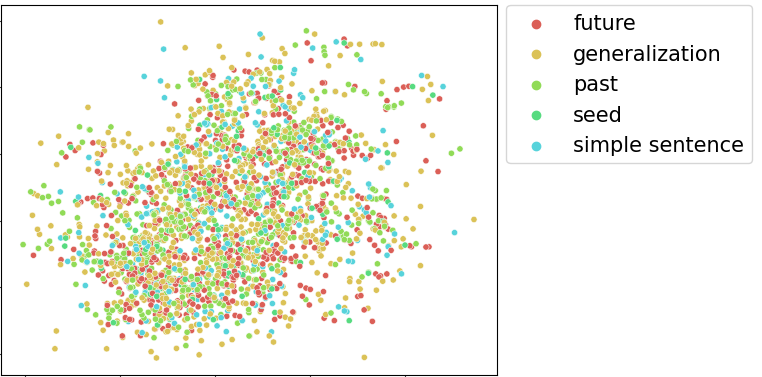
\includegraphics[scale=0.3]{figs/sbert_original.png}
    \caption{Visualization of five classes' SBERT sentence embeddings}\label{fig:sbert_original}
\end{figure}
\begin{figure}[htp]
    \centering
    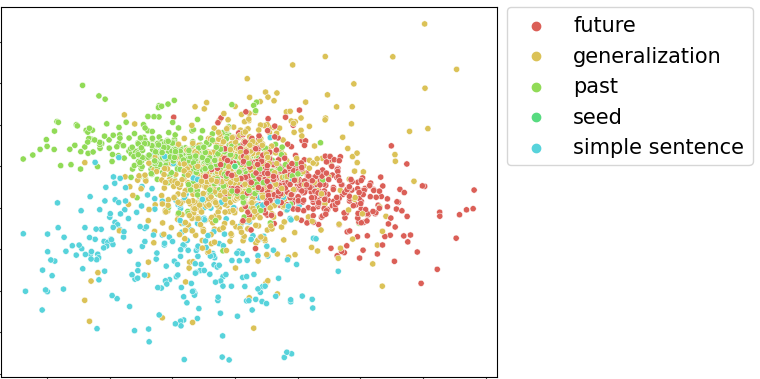
\includegraphics[scale=0.3]{figs/sbert_vis.png}
    \caption{Visualization of five classes' SBERT transformation embeddings (sentence embeddings minus their seeds).}\label{fig:sbert_vis}
\end{figure}
\begin{figure}[htp]
    \centering
    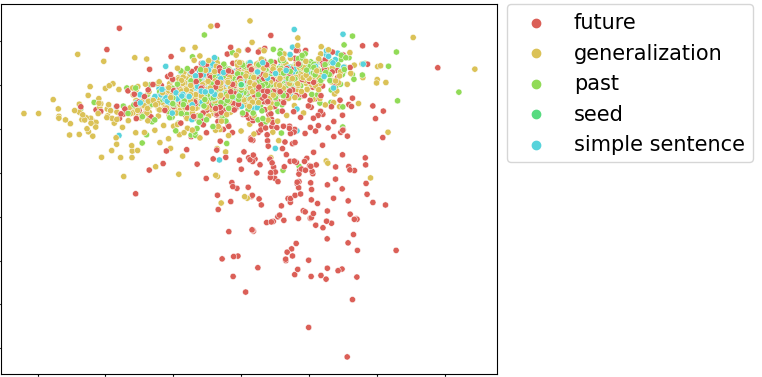
\includegraphics[scale=0.3]{figs/doc2vec.png}
    \caption{Visualization of five classes' doc2vec transformation embeddings (sentence embeddings subtract their seeds) }\label{fig:doc2vec_vis}
\end{figure}


\section{Test 1: Predication Capability of Transformation Embeddings}\label{sec:cosine}

This section tests whether the transformation vectors (sentence embeddings subtract the seed embedding) are capable to predict sentence embeddings for other seeds. We hypothesize that the transformation vectors of the same class share a similarity and are able to predict other sentence embeddings given the seed embedding. For instance, we assume that the following property holds: given two seed sentence embeddings $seed_i$ and $seed_j$, along with the future sentence embedding $future_i$, we can predict future sentence embeddings for $seed_j$ as equation \ref{eq:1} or \ref{eq:2}

\begin{equation}
\label{eq:1}
\small{ future_j = future_i - seed_i + seed_j}
\end{equation}
\begin{equation}
\label{eq:2}
 \small{future_j = Future\ Trans\ Embedding + seed_j}
\end{equation}

To test this hypothesis, We split each class to two parts: 80\% of the data for extracting transformation vectors ($sent_i$-$seed_i$) and calculating their average to predict sentence embeddings for the remaining 20\% data. We assess the performance by measuring the cosine similarity between the predicted sentence embeddings and the true sentence embeddings.


The results presented in Table \ref{cosine} indicate that the majority of the transformation classes achieved a cosine similarity score above 0.8. This score is higher than the benchmark range of 0.72-0.78, which was computed on the dataset with randomized seeds. 

These findings suggest that the predicted vectors closely approximate the true vectors in space, and the transformation vectors are relatively consistent for each transformation class.

The result also indicates that, however, the class `generalization' shows a lower cosine similarity score than the benchmark, which could be attributed to the fact that each seed contains multiple degrees of transformation for the `generalization' class. Some sentences are more generalized, while others are less so, and averaging 80\% of them may not be sufficient to predict the embeddings for sentences with varying transformation degrees.

\begin{table}[!htp]
\centering
\begin{tabular}{ c c }
\toprule
\vspace{0.1cm}
\textbf{class}&\textbf{cosine-sim} \vspace{0.15cm}\\ 
 \hline \\[-1.7ex]
\vspace{0.1cm} possibility &    0.936635 \\
\vspace{0.1cm} past & 0.930636 \\
\vspace{0.1cm} future &     0.923555 \\
\vspace{0.1cm} different meaning &    0.913798 \\
\vspace{0.1cm} nonsense &   0.901452 \\
\vspace{0.1cm} formal sentence &0.882741 \\
\vspace{0.1cm} minimal change & 0.866246 \\
\vspace{0.1cm} ban &  0.845272 \\
\vspace{0.1cm} paraphrase & 0.81659  \\
\vspace{0.1cm} nonstandard sentence & 0.812346 \\
\vspace{0.1cm} simple sentence &0.807523 \\
\vspace{0.1cm} opposite meaning &     0.748853 \\
\vspace{0.1cm} generalization & 0.697715 \\ 
\vspace{0.1cm} banchmark (randomized seeds) & 0.72-0.78 \\

\toprule
\end{tabular}
\caption{Cosine Similarity of predicted embeddings and true derivation sentence embeddings}
\label{cosine}
\end{table}

\section{Test 2: Clustering Test of Transformation Embeddings}\label{sec:cluster}
This section analyzes whether the transformation embeddings of the same class cluster together and are separated from other classes in space. Two unsupervised methods are utilized for testing purposes. In Section 5.1, we present an internal cluster validation test using the Calinski-Harabasz Index. In Section 5.2, we use Gaussian Mixture modeling to assess whether transformation classes can be separated with the Gaussian distribution-based method.

\subsection{Calinski-Harabasz Index}

The Calinski-Harabasz Index (Equation \ref{eq:3}) measures the ratio of between-cluster dispersion to inter-cluster dispersion. A higher value signifies well-separated clusters \cite{calinski1974dendrite}. In this study, we conducted pairwise testing of transformation embeddings generated by SBERT to assess the degree of separation between pairs of transformation classes in the vector space.
\begin{equation}
\label{eq:3}
  \scriptsize CH =\left[  {\frac {\sum_{k=1}^{K} n_k  \lVert c_k - c \rVert ^2}{K-1} }\right] /
 \left[ \frac{\sum_{k=1}^{K} \sum_{i=1}^{n_k}  \lVert d_i -c_k  \rVert ^2 }{N-K} \right] 
\end{equation}

We establish a benchmark for the CH Index by mixing up the seeds in the dataset, resulting in a range of 0.37 to 1.05. In our evaluation of SBERT transformation embeddings, we observe that 5 pairs fall below this benchmark (see Table \ref{CH_worst}). This indicates that the embeddings of `paraphrase', `minimal change', and `different meaning' are not separated from their seeds. Similarly, it suggests that the transformation embeddings of these three classes may not be distinguishable from one another.

\begin{table}[!htp]
\centering
\begin{tabular}{c c c}
\toprule
\vspace{0.1cm}
\textbf{class 1} &\textbf{class 2} &\textbf{CH index} \vspace{0.15cm}\\ 
 \hline \\[-1.7ex]
\vspace{0.1cm}paraphrase	& 	seed		& 0.77\\
\vspace{0.1cm}different meaning		&minimal change	&	0.80\\
\vspace{0.1cm}minimal change		&seed	& 0.88\\
\vspace{0.1cm}different meaning	&	seed	&	0.93\\
\vspace{0.1cm}different meaning	&	paraphrase	&	1.04\\
\toprule
\end{tabular}
\caption{5 pairs of classes with CH Index below the baseline}
\label{CH_worst}
\end{table}


\begin{table}[!htp]
\centering
\begin{tabular}{c c c}
\toprule
\vspace{0.1cm}
\textbf{class 1} &\textbf{class 2} & \textbf{CH index} \vspace{0.15cm}\\ 
 \hline \\[-1.7ex]
\vspace{0.1cm} ban	&	past	&	168.04 \\
\vspace{0.1cm} future	& past	&   147.48\\
\vspace{0.1cm} ban	& future	&	145.31 \\
\vspace{0.1cm} ban	& formal sentence	&112.28\\
\vspace{0.1cm} ban	& possibility	&102.32 \\

\toprule
\end{tabular}
\caption{5 pairs of transformation classes with the highest CH Index score}
\label{CH_best}
\end{table}

However, 66\% transformation pairs exhibit a significantly higher CH Index (above 10.00) than the benchmark. The classes with the highest separability from other classes include `ban', `future', `past', and `possibility'. The 5 best pairs are presented in Table \ref{CH_best}.

\subsection{Evaluating Sentence Embeddings with Gaussian Mixture}


This section analyzes the separability of transformation classes using the Gaussian Mixture model. It is a probabilistic model that assumes that each cluster follows a Gaussian (or normal) distribution and estimates the weight of
the density function for each cluster \cite{reynolds2009gaussian,5298967}. 

We assume that the transformation embeddings of two distinct classes should achieve high
accuracy with the Gaussian Mixture model if clusters are displayed in a Gaussian distribution
in space and are separable from each other.
We performed pairwise tests to assess the separability of labels and calculated the accuracy (F-score) of the GM clustered labels compared to the true labels.


Our evaluation results show that out of 78 pairs of derivation classes, 7 pairs
achieved an accuracy score above 90\%, 24 pairs above 80\%, and 47 pairs above
60\%, as depicted in Figure~\ref{fig:GM}.

In particular, the class `ban' demonstrates good separability with many other
classes, achieving an accuracy score of 0.982 with `past', 0.980 with `formal
sentence', 0.942 with `minimal change' etc. Additionally, our evaluation results reveal that tense-related classes are generally
well-separated, with an accuracy score of 0.90 for `past' and future' classes,
and an accuracy score of 0.924 for `simple sentence' and `future' classes.

\begin{figure}[htp]
    \centering
    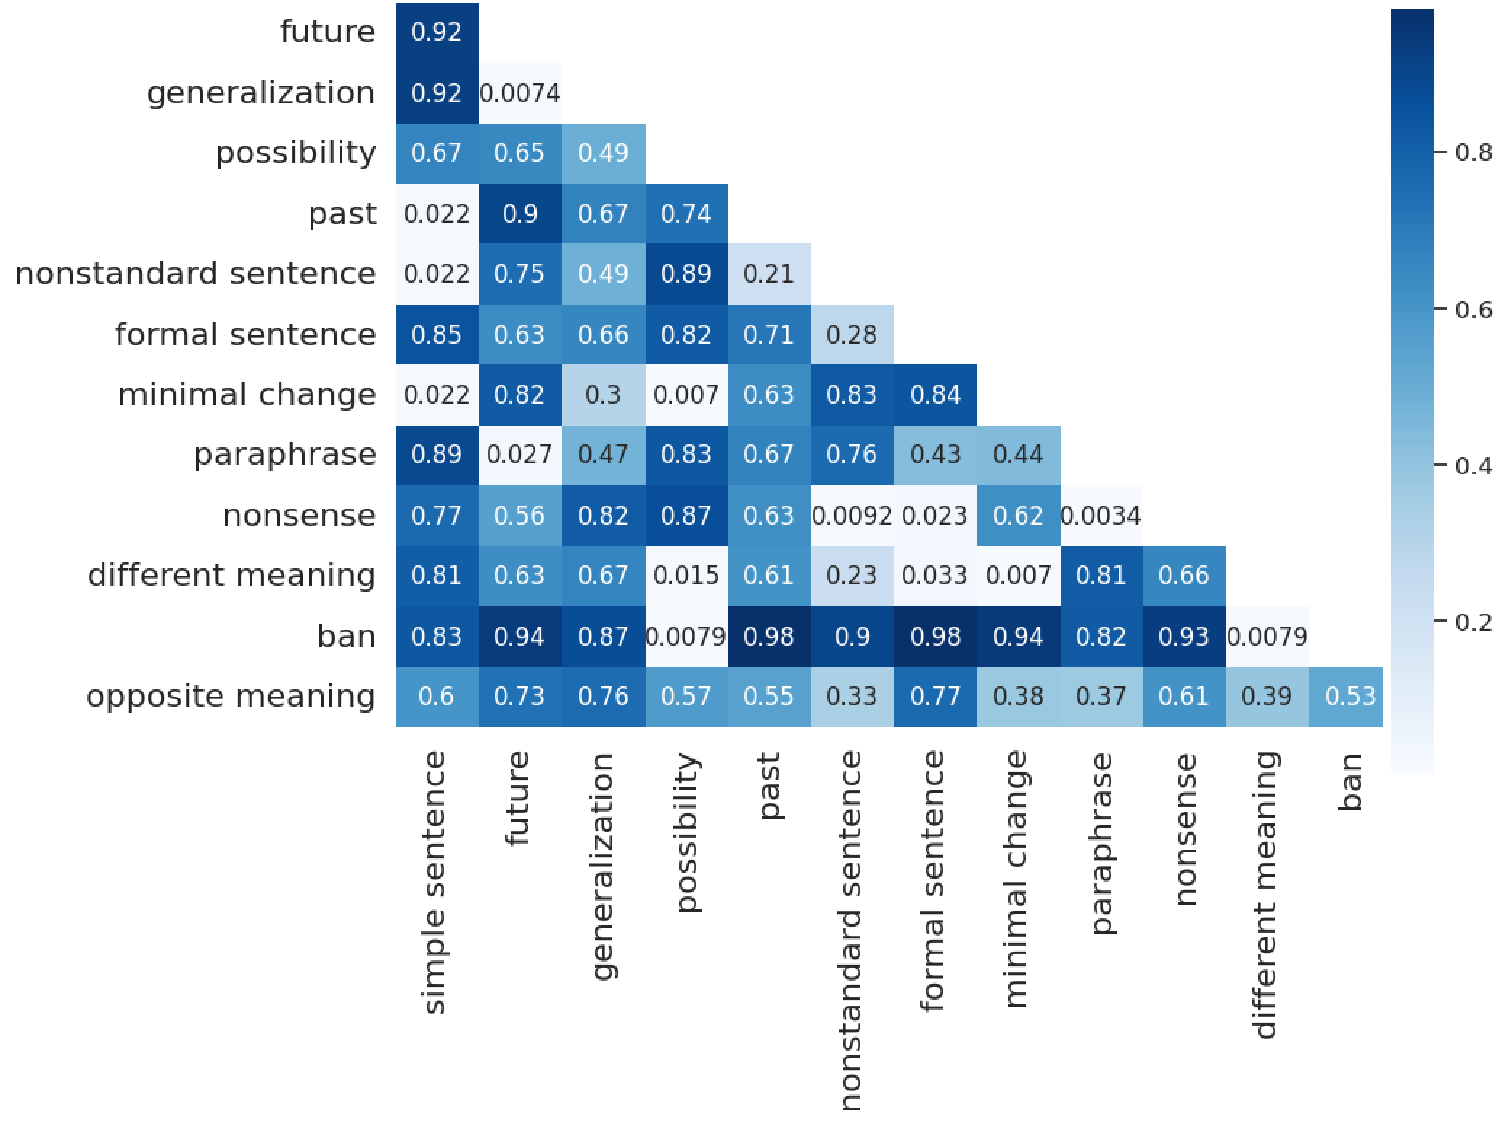
\includegraphics[scale=0.15]{figs/GM.png}
    \caption{Accuracy of class label prediction using Gaussian
    Mixture}\label{fig:GM}
\end{figure}

However, we realized the potential limitation of using this Gaussian Mixture accuracy as a measure of separability. The accuracy score from GM may be underestimated if two clusters are not normally distributed and the boundary between them is fuzzy.



%Enumeration of the tasks, for each task:
%  - starBriefly* describe the method used. Citing papers instead of
%  explaining.
%  - In case more information is needed (detailed method, implementation
%  notes), put it in an Appendix.
%  - Present results. Pinpoint the interesting stuff (in bold?)

\section{Test 3: Classification Tests of Embeddings}\label{sec:classification}

% Besides the already described embeddings in Section~\ref{sec:embeddings} XXX,  and several types
% bag-of-words (   {BOW}) vectors.  We experimented with two types of BOW
% vectors --- pure bow vector having ones at positions corresponding to words
% included in the given sentence (named  {bow}) and TF-IDF weighted bow
% vectors (named  {tfidf}).Dimensions of all embeddings are presented in
% Table~\ref{tab:embeddings_dim}.



In previous experiments, we utilized methods such as visualization, sentence embedding prediction, and clustering validation to assess the separability of classes. However, we observed that some classes may not be well-separated from other classes based on these methods. 

This section introduces more sophisticated supervised methods to further evaluate our sentence embeddings.
The classifiers include Random Forests, Support Vector Machine (SVM), and K-Nearest Neighbors (KNN). These methods have their own advantages: Random Forests use specific criteria and feature-based splitting to classify data \cite{breiman2001random, cutler2012random}, while SVM captures the decision boundary between two classes employing a hyperplane \cite{scholkopf1999advances, smola2004tutorial}. KNN uses a distance-based approach and classifies data based on the true labels of nearby data points. 

We intend to investigate whether these diverse methods could uncover any semantic information that might be encoded within the sentence embeddings.

In addition to the sentence embeddings from doc2vec and SBERT, we also included supervised SBERT sentence embeddings. They are  based on SBERT embeddings and further trained with MLP to predict class labels. Moreover, two lexical methods, namely bag of words (BoW) and term frequency-inverse document frequency (TF-IDF) weighted BoW, are also added to predicted class labels. The comparison with BoW and TF-IDF embeddings aimed to assess whether the classification performance is influenced by specific words that exclusively appear in a particular class. 

% In summary, our entire pipeline is as follows:
% \begin{enumerate}
%   \item For each embedding, we consider only a random sample with uniform
%     distribution of transformations and ignore the embeddings of the seed
%     sentences.
%   \item For each embedding and classifier we run a 5-fold cross-validated grid
%     search over several parameters, which gives us the best model for given
%     embedding.
%   \item We train each embedding on the classifier which performed the best
%     using cross-validation.
% \end{enumerate}

% More details about the pipeline can be found in
% Appendix~\ref{appendix:probing_method}.
% \subsection{Classifying sentence embeddings}
\subsection{Classification Performace of Varying Classifiers}

In this section, we compare three classifiers' performance in predicting transformation classes using two types of input: sentence embeddings (Figure \ref{fig:cls_gs_no_context_embed_comparison}) and transformation embeddings  (Figure \ref{fig:cls_gs_diff_embed_comparison}) in predicting transformation class labels.

\begin{figure}[htp]
  \centering
  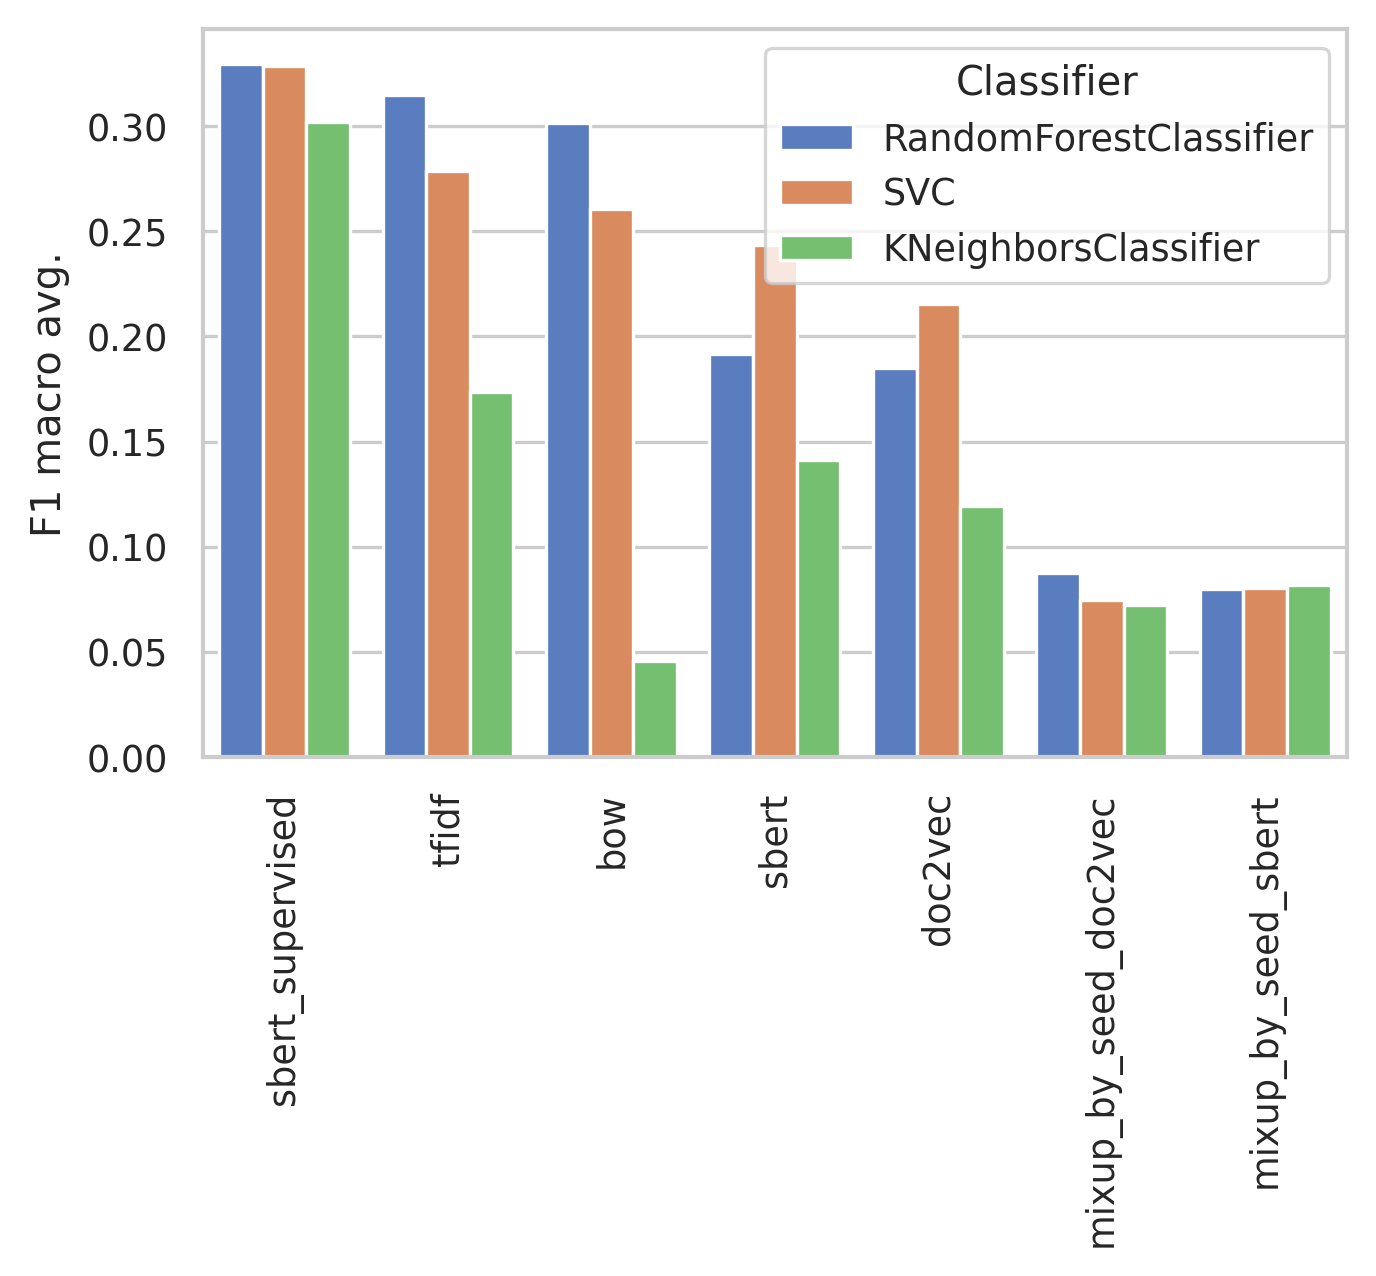
\includegraphics[width=0.5\textwidth]{./figs/cls_gs_no_context_embed_comparison.png}
  \caption{Averaged F1-macro scores of sentence embeddings from three classifiers. (The
  reported scores of  {sbert\_supervised} are computed as the mean
  of all SBERT supervised
embeddings.)}\label{fig:cls_gs_no_context_embed_comparison}
\end{figure}
\begin{figure}[htp]
  \centering
  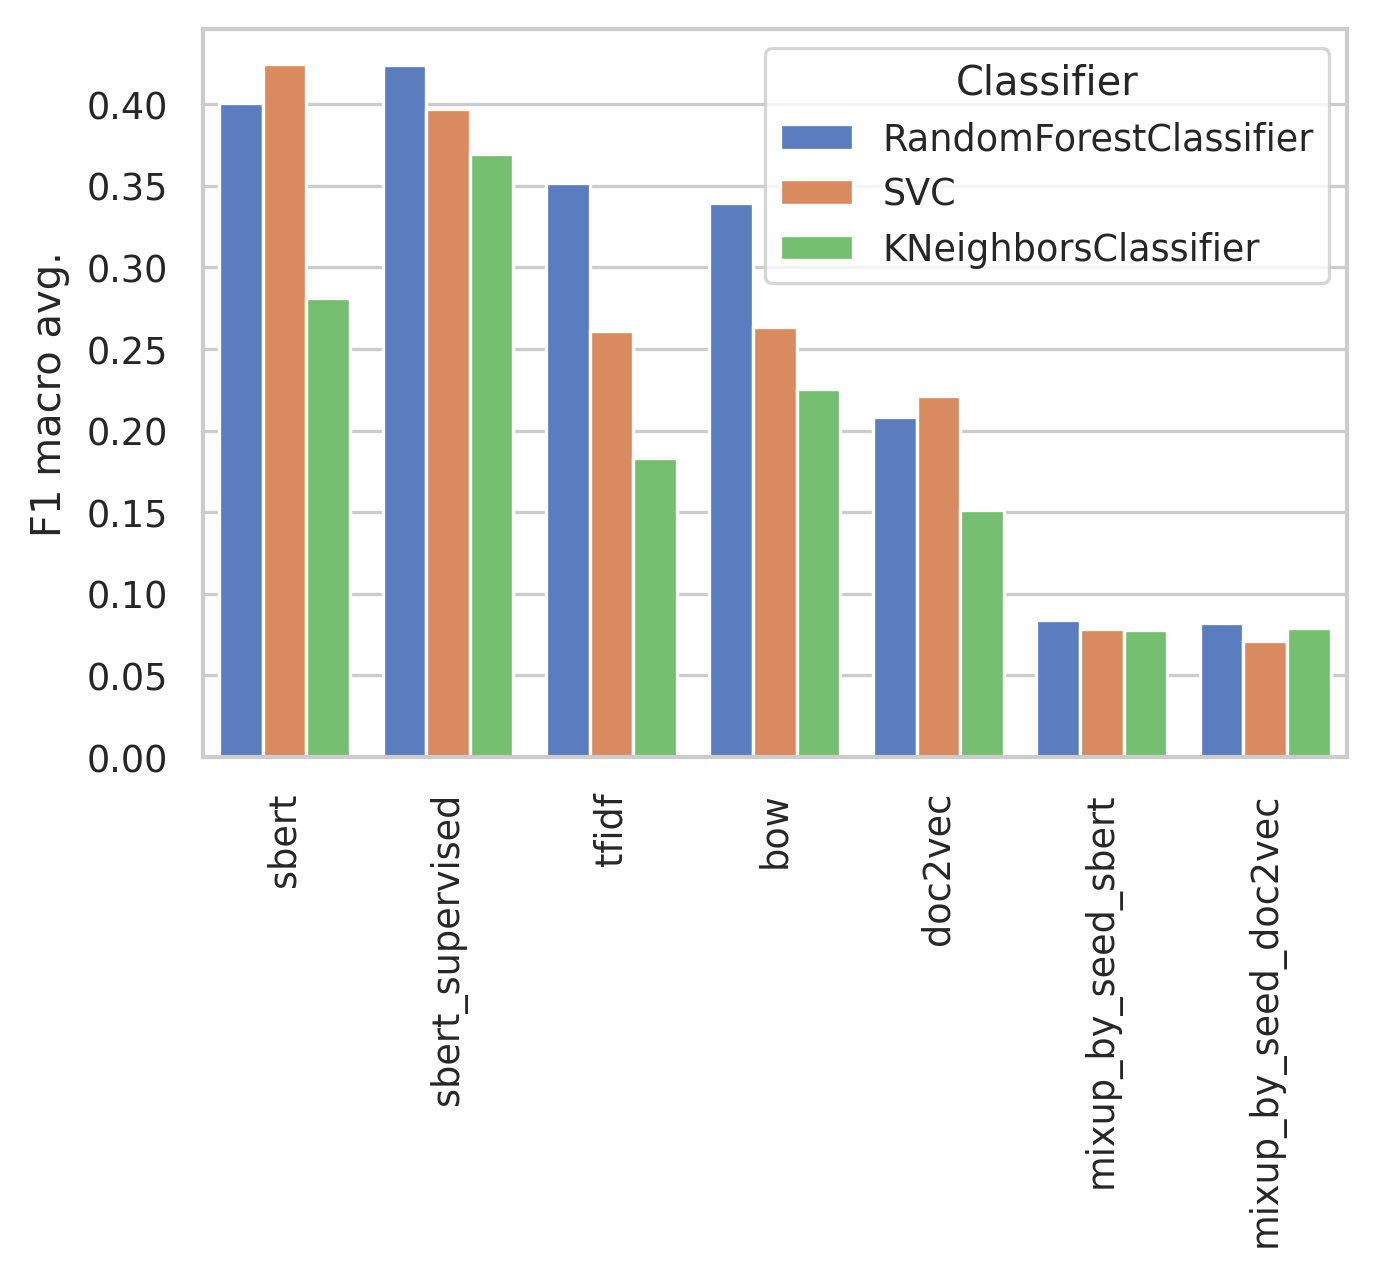
\includegraphics[width=0.5\textwidth]{figs/cls_gs_diff_embed_comparison.png}
  \caption{Average F1-macro scores for transformation embeddings from three classifiers.
  (The reported scores of  {sbert\_supervised} are computed as the mean of all
  SBERT supervised embeddings.
  }\label{fig:cls_gs_diff_embed_comparison}
\end{figure}

By comparing the performance of sentence embeddings (Figure \ref{fig:cls_gs_no_context_embed_comparison}) and transformation embeddings (Figure \ref{fig:cls_gs_diff_embed_comparison}), it can be observed that there is a significant difference in the performance of SBERT sentence embeddings and SBERT transformation embeddings. SBERT sentence embeddings perform even worse than TF-IDF. 

This suggests that embeddings that retain seed information introduce additional noise and make it more challenging to predict the correct classes. Subtraction of seed embeddings plays a crucial role in improving the prediction from SBERT embeddings. However, this distinction between sentence embeddings and transformation embeddings is less pronounced when using supervised SBERT embeddings. It suggests that preliminarily fine-tuning SBERT on the current task helps mitigate the impact of such noise.

The results of transformation embeddings in Figure \ref{fig:cls_gs_diff_embed_comparison} indicate that the embeddings of the best performance were generated by SBERT. Supervised SBERT embeddings demonstrated a significant advantage over unsupervised SBERT embeddings only when using k-nearest neighbors. This may reveal that KNN, the distance-based method relying on neighboring data points may not fully capture the relationships of the same class in high-dimensional space. The overall performance of KNN can be enhanced by using supervised trained embeddings as input.

Additionally, our findings suggest that TF-IDF weighted embeddings generally outperform the count-based Bag of Words (BoW) method. In the subsequent sections, we will mainly analyze predictions of SBERT and TF-IDF embeddings using the best-performing classifiers.

\subsection{Accuracy of Prediction of Class Labels}


In this section,  we analyze the prediction accuracy of SBERT and TF-IDF from sentence embeddings (Figure~\ref{fig:cls_gs_no_context_labels}) and transformation embeddings (Figure \ref{fig:cls_gs_diff_labels}). 

It is observed that performance from SBERT and TF-IDF display a correlation in both figures. A class that achieves a high F1 score with TF-IDF embeddings tends to have a high score with SBERT too. This finding suggests that the high accuracy score may be attributed to lexical factors. Specifically, the presence of certain words in the sentence may make the transformation classes more predictable. These results may also indicate that SBERT heavily relies on specific lexical information when encoding semantic information.

\begin{figure}[htp]
  \centering
  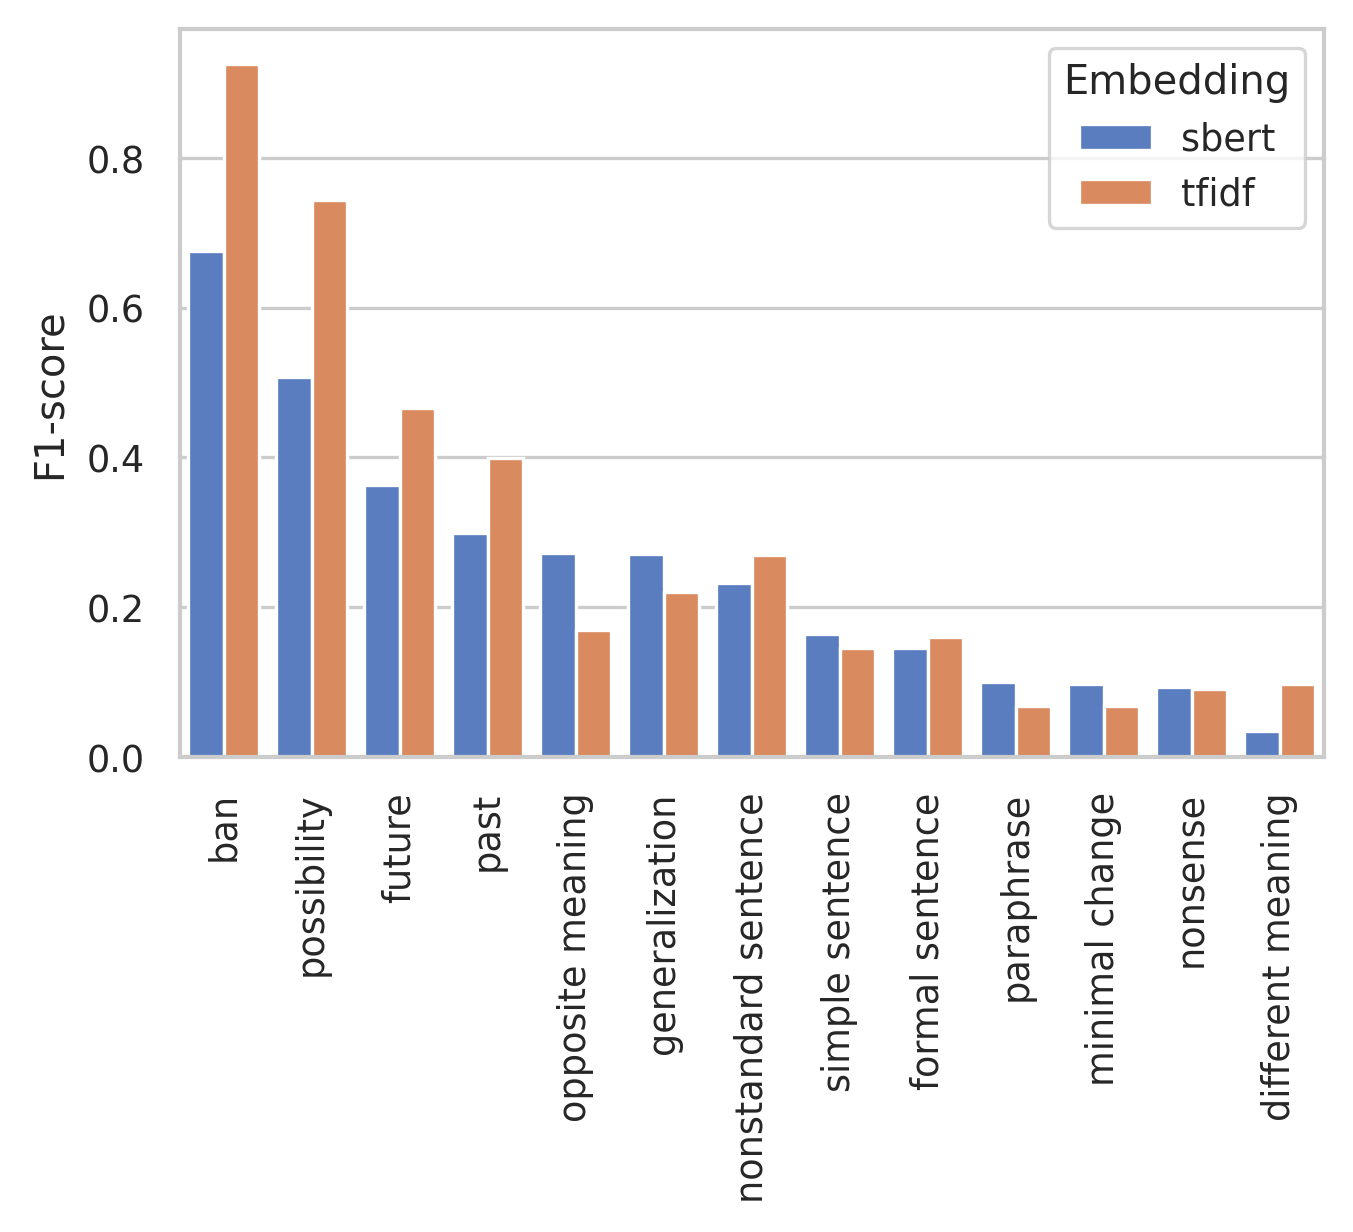
\includegraphics[width=0.5\textwidth]{figs/cls_gs_no_context_labels.png}
  \caption{F1 scores of sentence embeddings from the best classifier}\label{fig:cls_gs_no_context_labels}
\end{figure}
\begin{figure}[htp]
  \centering
  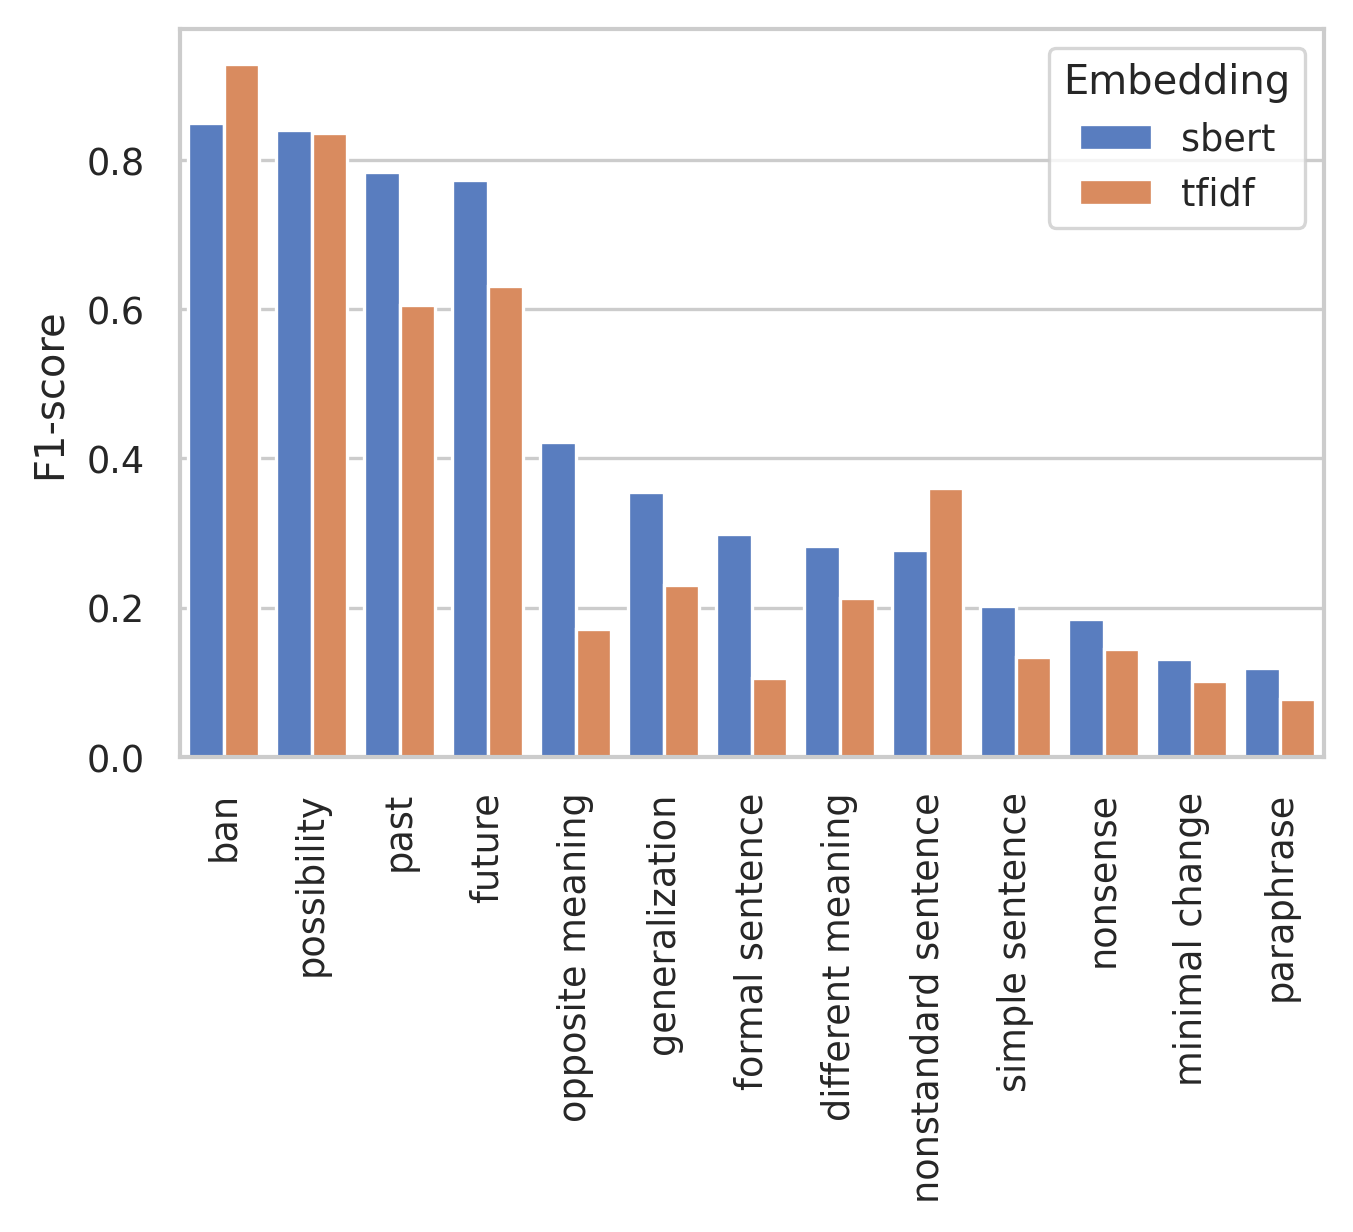
\includegraphics[width=0.5\textwidth]{./figs/cls_gs_diff_labels.png}

  \caption{F1 score of transformation embeddings from the
  best classifiers}\label{fig:cls_gs_diff_labels}
\end{figure}

Moreover, the results indicate transformation embeddings generally perform better than sentence embeddings, suggesting subtracting the corresponding seed embeddings improves the prediction accuracy for many classes. This tendency is pronounced for `different meaning', `future' and `past' (Figure \ref{fig:cls_gs_labels_context_diff}). 
\begin{figure}[htp]
  \centering
  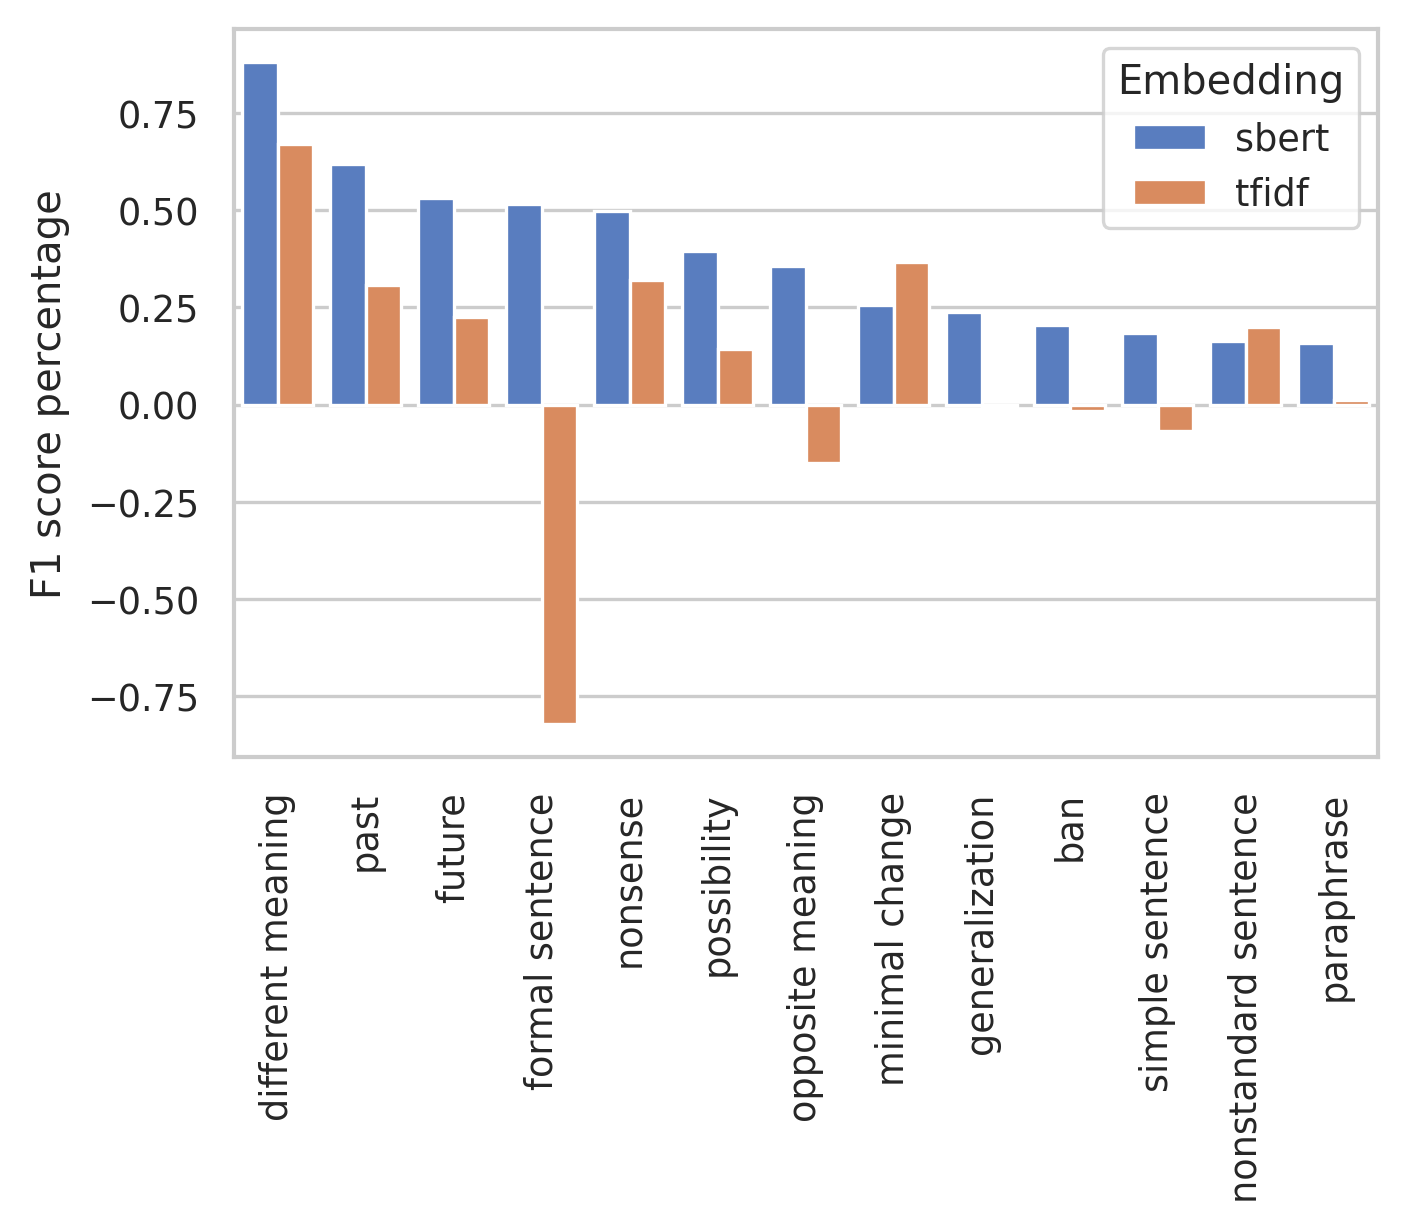
\includegraphics[width=0.5\textwidth]{figs/cls_gs_labels_context_diff.png}

  \caption{Updated performance by using transformation embeddings, compared with sentence embeddings from the best classifiers.}
 % The result is represented as a percentage of the score for transformation
 %  vectors.}
 \label{fig:cls_gs_labels_context_diff}.
\end{figure}
\begin{figure}[htp]
  \centering
  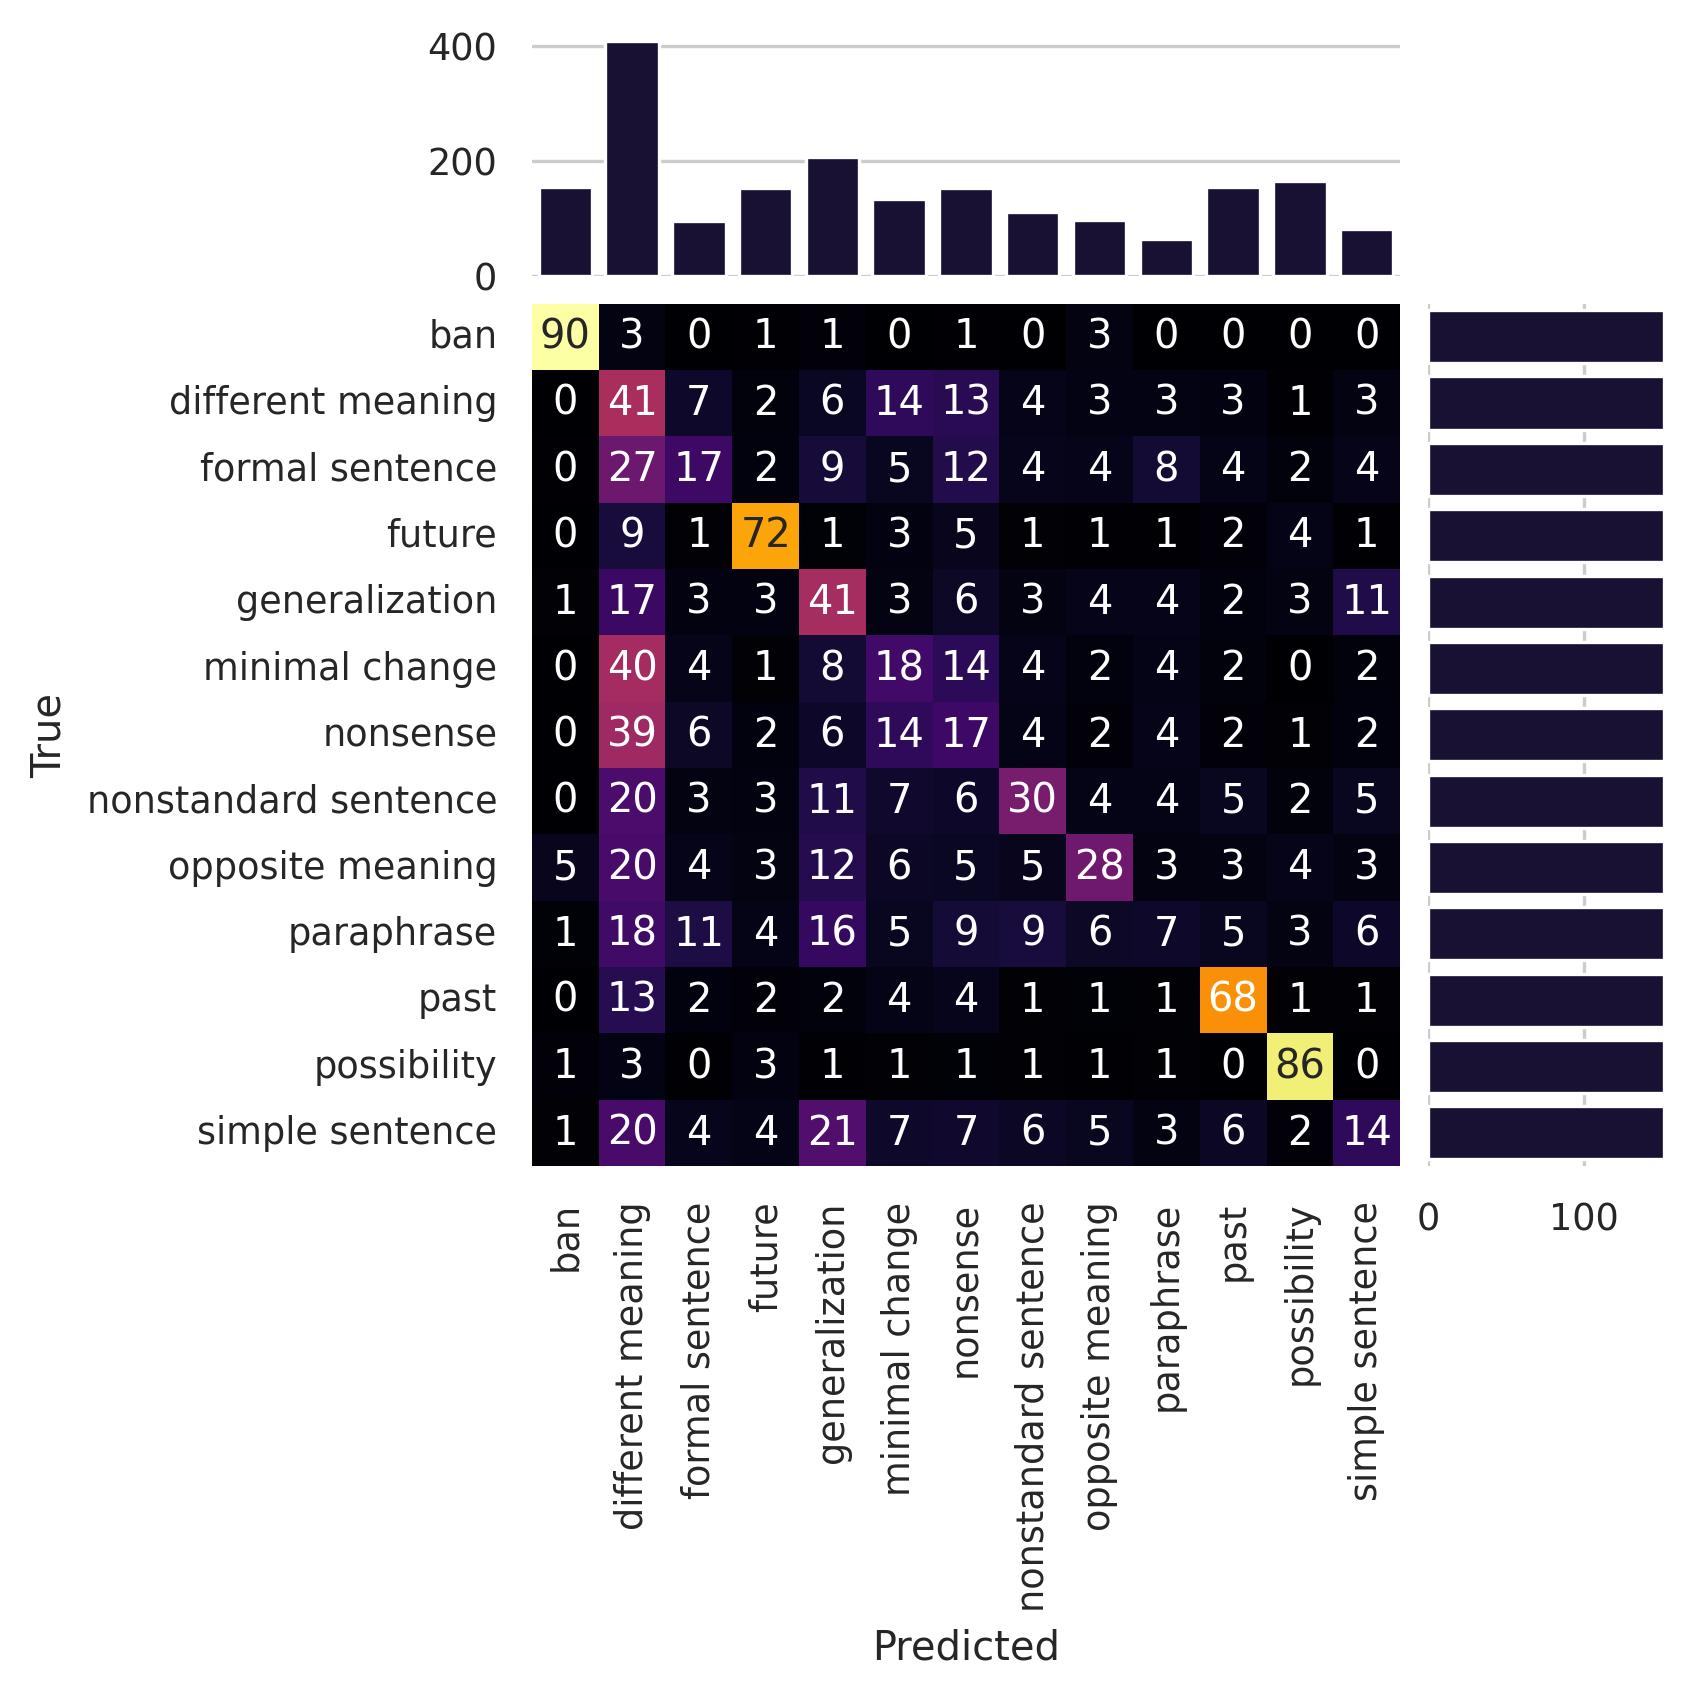
\includegraphics[width=0.5\textwidth]{./figs/cls_gs_diff_conf_mat.png}
  \caption{confusion matrix by summing up prediction from three sets of sentence embeddings (sbert, sbert\_supervised and TF-IDF) obtained from the best classifiers. The confusion matrix
  is normalized for each row.}
  %whereas the displayed true and predicted distributions are
  %not.}
  \label{fig:cls_gs_diff_conf_mat}
\end{figure}

In order to assess the difficulty of predicting specific transformation classes, we present a confusion matrix (Figure~\ref{fig:cls_gs_diff_conf_mat}) (based on the sum of predictions from the three best embeddings). The pairs with the least separability are `minimal change' vs. `different meaning' and `nonsense' vs. `different meaning'. Notably, the class `paraphrase' is frequently mispredicted (with an accuracy below 20\%.), and often gets mixed up with `simple sentence', `formal sentence', `nonsense', and `minimal change'.

% the classifiers' performance significantly drops in all cases except
% for the `ban' and the `possibility' transformations embedded with
% TF-IDF. This suggests that    `ban' and   `possibility' transformations
% can be easily identified from pure    {lexical} features and based on the
% sentence embedding only. the most seed-independent classes, followed by future and past. 
% While SBERT fails to encode this information into its
% embedding, it performs even better than TF-IDF when the embeddings of a
% sentence and its corresponding seed sentence are put into one context. As can
% be seen in Figure~\ref{fig:cls_gs_labels_context_diff}, this phenomena is
% pronounced mainly for   {different meaning} and   {past}
% transformations, where the inclusion of seed sentence's embedding on the input
% is responsible for over 80\% and 60\% of F1 score of the classifier. Overall
% SBERT's embeddings benefit from including the seed embedding to the input more
% than TF-IDF vectors.

% Moreover the BOW embeddings surpassed  doc2vec embedding,
% proving that for prediction of transformation, lexical features are more
% valuable than any information extracted by our trained Doc2vec model.

% TODO?: Should I mention the suprising performance of RandomForest on sparse
% embeddings?
 % In Figure~\ref{fig:cls_gs_diff_labels} we show the best performance of each class from  SBERT and pure lexical embedding  {tfidf}. Four
% transformation classes are being well-predicted by SBERT with the f1-score of around 0.80. 

\section{Conclusion}

Our study analyzed two sets of sentence embeddings: SBERT and doc2vec, and test tested them using the Costra corpus. We found that SBERT performed well in most tests, while the results from doc2vec were unsatisfactory.

Section \ref{sec:cosine} suggests that SBERT transformation embeddings (obtained by subtracting the seed embedding from the sentence embedding) from the corpus were capable of inferring the same transformation type for other seed sentences. However, the effectiveness of the predictions may be influenced by the degree of transformation. 

Regarding the separability of transformation classes, we conducted internal validity tests, unsupervised prediction, and supervised prediction of transformation labels. The results indicated that transformation embeddings generally perform better than original sentence embeddings. The experiment results also suggest that some classes exhibited higher separability than others, particularly those related to tense and transformation classes of `ban' and `possibility'. However, classes such as `minimal change', `paraphrase', and `different meaning' tend to be mixed up with each other. This tendency may also be consistent with the human judgment of transformation labels. In other words, these classes can be inherently difficult to distinguish.

One class that proved challenging for the embeddings to recognize, but not for humans is `non-sense'. This highlights the limitation of our sentence embeddings: although SBERT captures the meaning of individual words in the sentence, they lack the overall intelligence to understand the meaning of a sentence. The same finding is also supported by the positive correlation between SBERT and TF-IDF embeddings' performance, suggesting that sentence BERT embeddings, obtained by averaging pre-trained SBERT embeddings rely on the information of individual words. It also implies that inferring meaning beyond the word level is not be feasible using SBERT embeddings.



\bibliography{anthology}
\bibliographystyle{acl_natbib}

\clearpage
\appendix
\section{Other embeddings in the experiments}
\begin{table}[htp]
  \centering
  \begin{tabular}{l  c c}
    \toprule
    Embedding & Dimension & Sparseness\\
    \midrule
     doc2vec & 512 & 0\%\\
     SBERT & 384 & 0\%\\
     {bow} & 8374 & 99.89\%\\
     {tfidf} & 8374 & 99.89\%\\
    \bottomrule
  \end{tabular}
  \caption{Dimensionality and sparseness as the percentage of zeros of used
  embeddings.}\label{tab:embeddings_dim}
\end{table}
\section{SBERT embeddings}\label{appendix:sbert_embeddings}

For SBERT implementation we used the
\texttt{sentence\_transformers}\footnote{\url{https://www.sbert.net/}} python
library.

To produce sentence embeddings with SBERT, we chose pretrained model referred
to as `\textit{paraphrase-multilingual-MiniLM-L12-v2}'. It offers relatively
good scores for its size.

For the supervised SBERT sentence embeddings we list the hyperparameters used
in Table~\ref{tab:sbert_supervised_hparams}. Note that due to the small size of
training data, the model overfitted quickly. We therefore could afford to train
only for 4 epochs.

\begin{table}[htp]
  \centering
  \begin{tabular}{l c}
    \toprule
    Hyperparameter & Value\\
    \midrule
    epochs & 4 \\
    batch size & 8 \\
    warmup schedule & linear \\
    warmup steps & 10000 \\
    optimizer & AdamW \\
    weight decay & 0.1 \\
    learning rate & 2e-5 \\
    \bottomrule
  \end{tabular}

  \caption{Hyperparameters used to train SBERT for supervised
  embeddings}\label{tab:sbert_supervised_hparams}

\end{table}

\section{Probing method in detail}\label{appendix:probing_method}

For probing tasks whose results we described in
Section~\ref{sec:probing_results}, we used
\texttt{scikit-learn}\footnote{\url{https://scikit-learn.org/stable/}} python
package.

The grid searched parameters and classifiers are presented in
Table~\ref{tab:cls_gs_all_params}. We used cross-validated grid search, where
the performence of a set of parameters is evaluated using cross validation. For
all cross validations (both within and outside of grid search) we used
\texttt{StratifiedGroupKFold}, where seed identifiers were used as groups. This
caused the folds to be stratified as well as sharing as few common seed
sentences as possible.

\begin{table*}[htp]
  \centering

  \begin{tabular}{l l l}
    \toprule
    Classifier & Hyperparameter & Values searched \\
    \midrule
    \multirow{3}{13em}{\Cls{RandomForestClassifier}}
    & \texttt{n\_estimators} & 50, 100, 200 \\
    & \texttt{max\_depth} & 2, 5, 25, None \\
    & \texttt{min\_samples\_split} & 2, 10, 20 \\
    \midrule
    \multirow{2}{13em}{\Cls{SVC}*}
    & \texttt{kernel} & rbf, linear \\
    & \texttt{gamma} & auto, scale\\
    \midrule
    \multirow{2}{13em}{\Cls{KNeighboursClassifier}*}
    & \texttt{n\_neighbours} & 3, 5, 10\\
    & \texttt{weights} & uniform, distance\\
    \bottomrule
  \end{tabular}

  \caption{Classifiers and hyperparameters grid search for probe tasks. All are
  named equally as in the \texttt{scikit-learn} python package. *Embeddings
  were first scaled to have zero mean and unit
  variance.}\label{tab:cls_gs_all_params}

\end{table*}

We report the best performing set of parameters for each classifier in
Tables~\ref{tab:cls_gs_best_params_SVC},~\ref{tab:cls_gs_best_params_RandomForestClassifier}~and~\ref{tab:cls_gs_best_params_KNeighborsClassifier}

\begin{table*}[htp]
  \centering
  \begin{tabular}{lcccc}
\toprule
&  & \texttt{gamma} & \texttt{kernel} \\
Context & Embedding &  &  \\
\midrule
\multirow[c]{2}{*}{diff} & \Embed{doc2vec} & auto & rbf \\
& \Embed{sbert} & auto & rbf \\
\noalign{\smallskip}
\cline{1-4}
\noalign{\smallskip}
\multirow[c]{4}{*}{no-context} & \Embed{doc2vec} & auto & rbf \\
& \Embed{sbert} & auto & rbf \\
& \Embed{sbert\_supervised\_0} & auto & rbf \\
& \Embed{sbert\_supervised\_2} & auto & rbf \\
\bottomrule
\end{tabular}


  \caption{Best parameters for \Cls{SVC}
  classifier.}\label{tab:cls_gs_best_params_SVC}

\end{table*}

\begin{table*}[htp]
  \centering
  \begin{tabular}{lccccc}
\toprule
&  & \texttt{max\_depth} & \texttt{min\_samples\_split} & \texttt{n\_estimators} \\
Context & Embedding &  &  &  \\
\midrule
\multirow[c]{9}{*}{diff} & \Embed{bow} & 25 & 20 & 200 \\
& \Embed{mixup\_by\_seed\_doc2vec} & None & 5 & 200 \\
& \Embed{mixup\_by\_seed\_sbert} & 25 & 5 & 200 \\
& \Embed{sbert\_supervised\_0} & None & 5 & 200 \\
& \Embed{sbert\_supervised\_1} & None & 5 & 200 \\
& \Embed{sbert\_supervised\_2} & 25 & 10 & 200 \\
& \Embed{sbert\_supervised\_3} & None & 5 & 200 \\
& \Embed{sbert\_supervised\_4} & None & 10 & 100 \\
& \Embed{tfidf} & None & 20 & 200 \\
\noalign{\smallskip}
\cline{1-5}
\noalign{\smallskip}
\multirow[c]{6}{*}{no-context} & \Embed{bow} & 25 & 10 & 200 \\
& \Embed{mixup\_by\_seed\_doc2vec} & None & 20 & 50 \\
& \Embed{sbert\_supervised\_1} & 25 & 10 & 50 \\
& \Embed{sbert\_supervised\_3} & 25 & 10 & 100 \\
& \Embed{sbert\_supervised\_4} & 25 & 5 & 50 \\
& \Embed{tfidf} & 25 & 10 & 200 \\
\bottomrule
\end{tabular}


  \caption{Best parameters for \Cls{RandomForestClassifier}
  classifier.}\label{tab:cls_gs_best_params_RandomForestClassifier}

\end{table*}

\begin{table*}[htp]
  \centering
  \begin{tabular}{lcccc}
\toprule
&  & \texttt{n\_neighbors} & \texttt{weights} \\
Context & Embedding &  &  \\
\midrule
no-context & \Embed{mixup\_by\_seed\_sbert} & 5 & distance \\
\bottomrule
\end{tabular}


  \caption{Best parameters for \Cls{KNeighboursClassifier}
  classifier.}\label{tab:cls_gs_best_params_KNeighborsClassifier}

\end{table*}

% chosen parameters




\end{document}